\chapter{Knots and Knot diagrams}\label{chap:knots-and-knot-diagrams}
\setlength\epigraphwidth{.7\textwidth}
\epigraph{and an ocean tumbled by with a private boat for Max\\
and he sailed off through night and day\\
and in and out of weeks\\
and about over a year\\
to where the wild things are.}{---Maurice Sendak, \emph{Where the Wild
Things Are}}
The material here is targeted at readers with a basic background in
topology. Experts are advised to skim (or even skip).

% Before we start, a quick note for the reader who is already
% experienced with knot theory:\vspace{.5em}
% % \begin{adjustwidth}{1em}{}
%   \begin{leftbar}
%     \textbf{A word on convention:} In the below, we will define a
%     \emph{knot} to be an embedding of a circle into an arbitrary
%     topological space. This represents a significant break from the
%     usual convention, which is to define a knot as an embedding into
%     either $\RR^3$ or $S^3$. The justification for this decision is
%     that we want to avoid backpedalling when defining \emph{virtual
%       knots}.\\

%     \noindent \textbf{Recommendation on what to read:} We define knots
%     in \cref{sec:KnotDef} and ambient isotopy in \cref{sec:KnotEq};
%     both of these can probably be skipped. In \cref{sec:KnotDiags}, we
%     define the concept of a \emph{diagramming scheme}, which isn't
%     emphasized in most resources. We recommend even the experienced
%     reader skim this part.
%   \end{leftbar}
% % \end{adjustwidth}
% Anyways, on to the introduction.

% {\color{red} Come back and revise to not rely on talking about 3D
%   objects. Also come back and add page references for things}

Knots are fundamentally 3D objects. Studying 3D objects can be hard,
so we'd much rather work with 2D representations if possible.
\emph{Knot diagrams} facilitate this process. The idea is that placing
strict requirements on what we call a ``knot diagram'' allows us to
translate results about these 2D objects to ones for the actual knots.
It's important to be very explicit about how we do this, as the
restrictions we place on our diagrams will dictate what families of
knots we can study with them. The goal for this chapter is to give the
reader intuition for this process.

Our exposition is structured as follows: First, we give the formal
definition of a knot and discuss some of its equivalent versions
(\cpagerefrange{sec:KnotDef}{sec:KnotEq}). We also offer some
intuition for why each requirement in the definition is necessary.
Next, we introduce the standard equivalence relation on knots, which
is known as \emph{ambient isotopy}
(\cpagerefrange{sec:KnotEq}{sec:polygonal-knots}). In doing so, we
first examine two other definitions of equivalence that seem
reasonable but turn out to be flawed (\emph{homeomorphism} and
\emph{non-ambient isotopy}, respectively). Finally, we define
\emph{knot categories} and their associated \emph{diagram categories}.
This offers a nice segue into the next chapter, which discusses the
most common knot category/diagram category pair: \emph{polygonal
  knots} and \emph{regular diagrams}.

\section{Definition of a Knot}\label{sec:KnotDef}
We have to define knots before defining knot diagrams. But to make our
the definition tangible, we need to draw pictures. Hence, we'll have
to make use of knot diagrams before we've actually defined them. The
reader shouldn't worry about this, since it turns out most of the
things we'll need to address in our formal treatment of knot diagrams
are edge cases.

Recall, the intuitive description of a knot that we gave earlier
(\cref{fig:knotcons} on \cpageref{fig:knotcons}) involved taking a
rope, twisting it around in space, and then fusing the ends to get a
closed loop. Importantly, the strand remained ``unbroken'' (in the
sense that there were no cuts in the rope anywhere), and never passed
through itself. This is encoded in the following definition.
\begin{definition}[Topological Knot]\label{def:GenKnotInt}
  Let $(X, \ms T)$ be a topological space. Then a \emph{knot} is a
  continuous map $K : [0,1] \to X$ such that $K$ is injective on
  $[0,1)$, and $K(0) = K(1)$.
\end{definition}
% {\color{red} Let's maybe revise this to be in terms of embeddings}
We'll discuss the importance of the choice of codomain $(X,\ms T)$
later on. But first, to build intuition, we'll restrict our analysis
to the case where $(X, \ms T)$ is $\RR^3$ with the standard topology
(denoted $\ms T_{\rm std}$). This gives us the field of
\emph{classical knot theory}, whose objects of study are
\emph{classical knots}.\footnote{Some authors choose to use $S^3$
  instead of $\RR^3$ because $S^3$ is compact. We won't worry about
  this distinction today.% The interested reader might look into the
  % \emph{Alexandroff extension}, which gives the relationship between
  % $\RR^3$ and $S^3$.
}

\subsection{Classical Knots}
Most of the intuition from $\RR^3$ generalizes to the other choices of
$(X, \ms T)$ we'll be interested in. We just chose to examine the
special case of \emph{classical knots} first to decrease the number of
moving parts in the definition.
\begin{definition}[Classical Knot]\label{def:ClassKnotInt}
  A \emph{classical knot} is a topological knot where $(X,\ms T)$ is
  $(\RR^3, \ms T_{\rm std})$.%  More explicitly, a classical knot is a
  % continuous map $K : [0,1] \to \RR^3$ such that $K$ is injective on
  % $[0,1)$ and $K(0) = K(1)$.
\end{definition}
\begin{aside}
  The choice $[0,1]$ is arbitrary; we could modify our definition to
  use any interval $[a,b]$ and still get a topologically equivalent
  framework. Similarly, choosing $K$ to be injective on $[0,1)$ vs
  $(0,1]$ is also arbitrary since we have $K(0) = K(1)$. We'll remove
  these annoyances later with an equivalent definition in terms of
  $S^1$, but first, let's talk about what this definition is doing.
\end{aside}

First, the codomain is $\RR^3$, so we get an object that lives in 3D
space like we want. Second, we do indeed get a ``loop;'' we can think
of the the domain $[0,1]$ as parameterizing how far along a 1D path we
are.\footnote{You might wonder if space-filling curves would cause
  problems here. It turns out they won't, since we would need to
  loosen one of \{injectivity, continuity\} to get one.} As an
example, if we had $K(t) = (\cos(2\pi t), \sin(2\pi t), 0)$, then
looking down along the $z$ axis and playing time forwards, we would
see something like the following:
\begin{figure}[H]
  \centering
  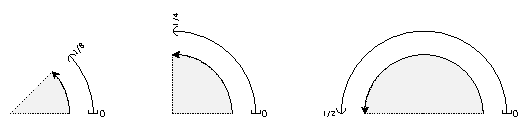
\includegraphics[scale=1.4]{figures/background/dist-along-knot.pdf}
  \caption{Analogy for the domain}
  \label{fig:DomainAnalogy}
\end{figure}
\noindent Here, the inner ring shows $K(t)$ itself, while the outer
ring is just showing us a reminder of what the corresponding values of
$t$ are.

Next, note that requiring $K$ be \emph{continuous} and $K(0) = K(1)$
prevents us from getting any ``breaks'' in the strand (a rope wouldn't
make a good knot if it had a cut in it); see \cref{fig:KnotBreak}
below. Similarly, the injectivity condition prevents us from getting
self-intersections in our rope; see
\cref{fig:SelfIntersect} below.\\
\begin{minipage}{.49\linewidth}
  \begin{figure}[H]
    \centering
    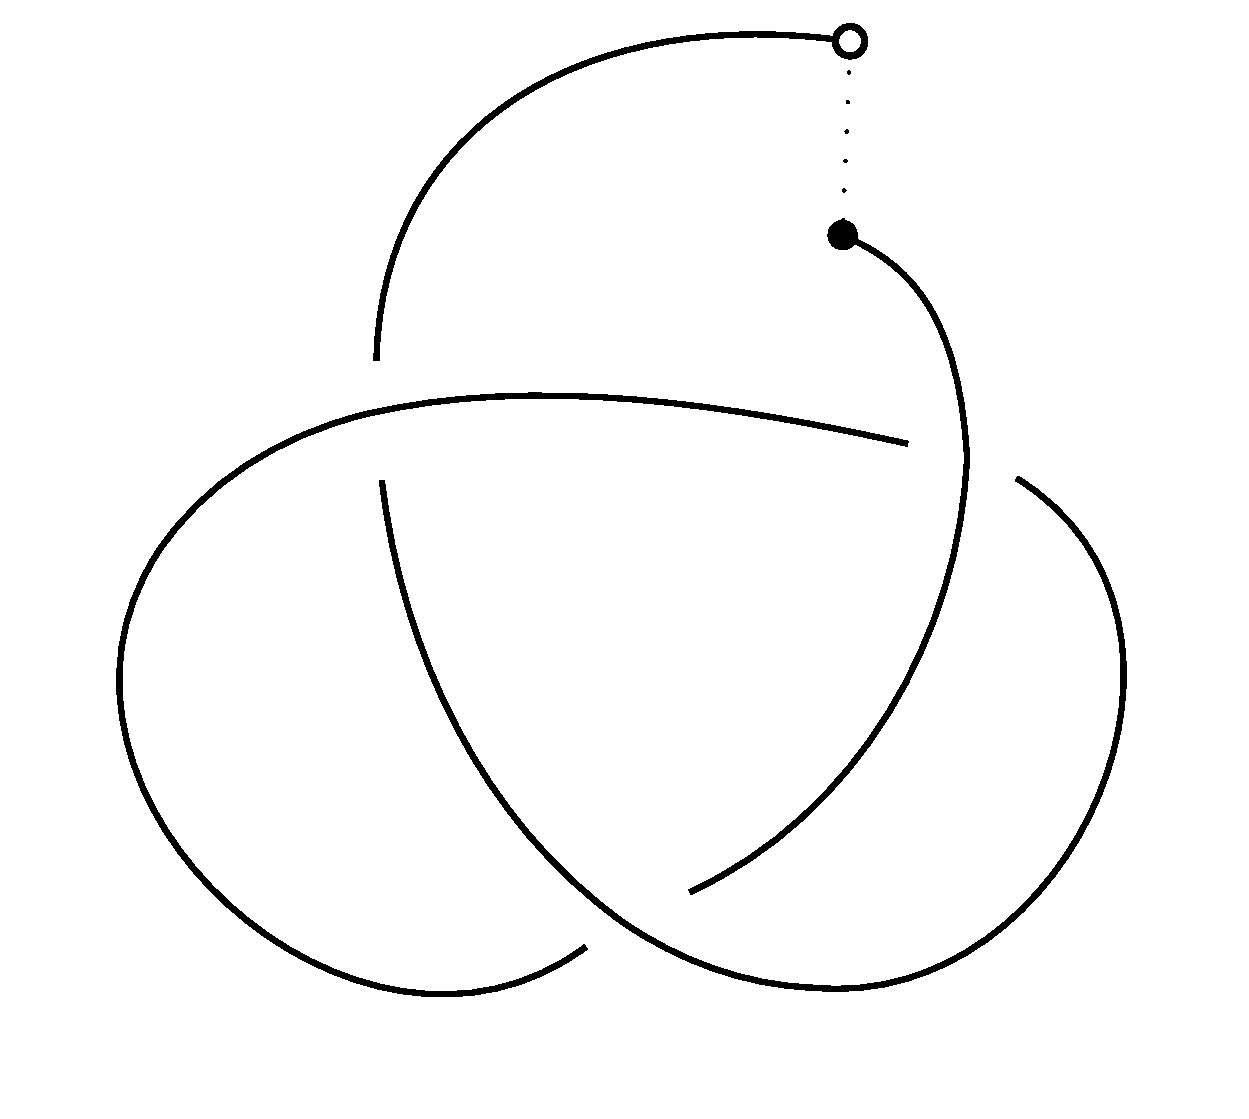
\includegraphics[scale=.15]{figures/background/broken-trefoil.pdf}
    \caption{A ``knot'' with a break in it}
    \label{fig:KnotBreak}
  \end{figure}
\end{minipage}
\begin{minipage}{.49\linewidth}
  \begin{figure}[H]
    \centering
    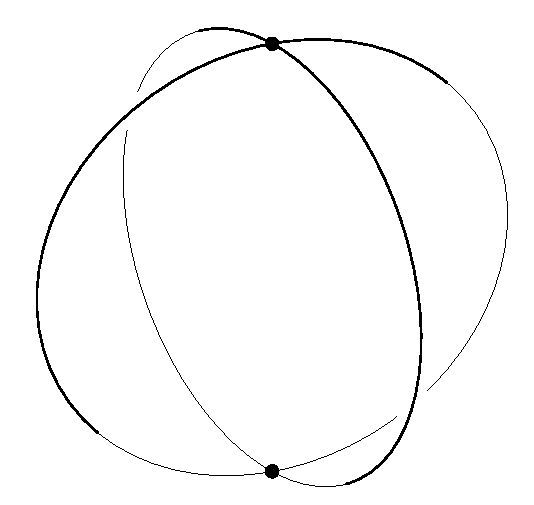
\includegraphics[scale=.3]{figures/background/self-intersect.pdf}
    \caption{A ``knot'' with points of self-intersection (black)}
    \label{fig:SelfIntersect}
  \end{figure}
\end{minipage}\\[1em]
To see that the ``knot'' in \cref{fig:SelfIntersect} really \emph{can}
be realized as a continuous function $K : [0,1] \to \RR^3$ (and thus
the injectivity condition is strictly necessary), consider the
following construction: % {\color{red} rewrite me}
\begin{figure}[H]
  \centering
  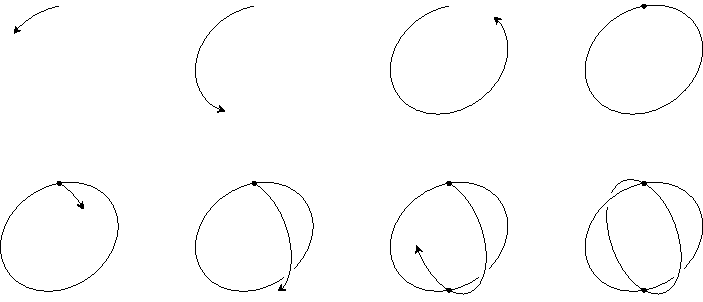
\includegraphics[scale=.8]{figures/background/self-intersect-cons.pdf}
  \caption{Example of how we'd construct the self-intersecting ``knot''}
\end{figure}
\noindent Hence we see we need all of the pieces of the definition
given.
% \noindent\hrulefill

\subsection{Equivalent Definition in terms of $S^1$}
% {\color{red} Maybe we also wanna talk about general $[a,b]$}

Okay: \cref{def:ClassKnotInt} is fine and intuitive, but as alluded to
before, it can be written more succinctly. In particular, the whole
``injective on $[0,1)$ and $K(0) = K(1)$ except you could also use
$(0,1]$'' part can be done away with by gluing the ends of $[0,1]$
together to get a circle. This motivates the second definition, which
is more commonly used.

\begin{definition}[Classical Knot, redux]\label{def:ClassKnotS1}
  A \emph{knot} is an injective, continuous map $K : S^1 \into \RR^3$.
\end{definition}
Note, since we already identify $0$ and $1$ in $S^1$, we don't have to
state the extra injectivity conditions. We'll use this definition
throughout the rest of this document.%  {\color{red} Come back and talk
  % about how we did away with the arbitrary interval part by
  % precomposing with a homeomorphism.}

It is straightforward to show that this is equivalent to the previous
definition. Here's the strategy: let $K : [0,1] \to \RR^3$ be a knot
(in the sense of the first definition), and let $\pi$ be the quotient
map $\pi : [0,1] \to [0,1]/\set{0 \sim 1}$. Then show that there
exists a unique continuous $K' : S^1 \into \RR^3$ such that the
following diagram commutes:
\begin{figure}[H]
  \centering
  \begin{tikzpicture}
    \node (a) at (-1.5,0) {$[0,1]$};
    \node (b) at (0,-1.5) {$S^1$};
    \node (c) at (1.5, 0) {$\RR^3$};

    \draw[-latex] (a) -- (b) node[midway, below left] {$\pi$};
    \draw[-latex] (a) -- (c) node[midway, above] {$K$};
    \draw[-latex] (b) -- (c) node[midway, below right] {$K'$};
  \end{tikzpicture}
  \caption{Commutative diagram}
\end{figure}
This is straightforward enough that it might seem silly to state
explicitly, but it is cool to see it in action. Check out
\href{https://youtu.be/7cDroN4n8EQ}{https://youtu.be/7cDroN4n8EQ} for
an example animation.
\begin{example}
  The following is a knot known as $(7,2)$.
  \begin{figure}[H]
    \centering
    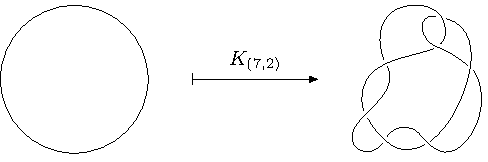
\includegraphics{figures/background/embed-72.pdf}
    \caption{The $(7,2)$ knot}\qedhere
  \end{figure}
  \label{ex:72knot}
\end{example}
The name $(7,2)$ convention comes from the fact that 7 is the minimum
number of crossings we can have in a diagram for the knot. The 2 is
just a label dictated by convention so that we know \emph{which} of
the 7-crossing knots we're dealing with.\footnote{For a gallery of the
  so-called \emph{prime} knots up to a given crossing number, see
  \href{http://katlas.math.toronto.edu/wiki/The_Rolfsen_Knot_Table}{http://katlas.math.toronto.edu/wiki/The\_Rolfsen\_Knot\_Table}}

There is a sense in which knots act like homeomorphims. In particular,
for a knot $K$, the \emph{image} of $S^1$ under $K$ is still a closed
loop (and in fact, this loop is homeomorphic to $S^1$). But since $K$
is not a bijection ($K$ is not not onto $\RR^3$), we can't call it a
homeomorphism. We can, however, call it an embedding.
\begin{definition}[Embedding]
  Let $(X,\ms T)$, $(Y, \ms S)$ be topological spaces, and let $f : X
  \to Y$. Then we say $f$ is an \emph{embedding} iff $f$ is a
  homeomorphism between $X$ and $f(X)$, where $f(X)$ is given the
  subspace topology from $Y$.
\end{definition}

\begin{proposition}\label{prop:knots-are-embeddings}
  Let $K : S^1 \into \RR^3$ be a knot. Then $K$ is an
  \emph{embedding}.
\end{proposition}
\begin{proof}
  % The following is based on a stackexchange thread. \footnote{See
  %   \href{https://math.stackexchange.com/questions/474693/if-we-have-an-embedding-fx-rightarrow-a-where-a-subset-y-do-we-have-to}{https://math.stackexchange.com/questions/474693/if-we-have-an-embedding-fx-rightarrow-a-where-a-subset-y-do-we-have-to}}

  We want to show $K$ is a homeomorphism between $X$ and $K(X)$. Note,
  any injective function is bijective with its image, so $K$ is a
  bijection between $X$ and $K(x)$. Now, the definition of a knot
  guarantees $K$ is continuous. Given these conditions, one can show
  that it suffices to prove $K$ is a closed map (i.e.\ image of a
  closed set is closed).

  Let $A \subseteq S^1$ be closed. Since $S^1$ is compact, it follows
  that $A$ is compact. Since $K$ is continuous, it follows that $K(A)$
  is compact. Now, since $\RR^3$ is Hausdorff, all compact sets are
  closed. Hence $K(A)$ is closed, so $K$ is a closed map, and thus a
  homeomorphism (as desired).
\end{proof}

\subsection{Other Codomains}
We want to take a moment to stress that the choice of codomain is a
hugely important factor in determining the behavior of our knots.
Knottedness (as a general phenomenon) \emph{fundamentally} arises out
from taking a small space and trying to find ways to fit into a
slightly larger one. Here, we've taken $S^1$ (a 1-manifold) and stuck
it into $\RR^3$, but one might wonder whether we'd get different
theories if we tried, say, $\RR^2$, $\RR^4$, or $\RR^n$.

It turns out that we do. In both $\RR^2$ and $\RR^4$, \emph{all} knots
turn out to be equivalent to each other. The intuition is a bit
different in $\RR^2$ than in $\RR^4$, however. We'll examine the
$\RR^2$ case in more detail during \cref{chap:ambient-isotopy-in-r2},
but the loose idea is that $\RR^2$ ``confines'' our embedded copy of
$S^1$ too tightly to allow it to get all tangled up (indeed, the
string can't cross itself when restricted to $\RR^2$). In $\RR^4$, we
see the opposite phenomenon. Because we have a whole extra spatial
dimension to work with, the string can never quite get ``stuck'' on
itself in $\RR^4$ --- there's always a sneaky way to get around the
barrier.\footnote{We have some slides posted at
  \url{https://bedmathandbeyond.xyz/files/kaestner-brackets.pdf} with
  a small visualization, but the reader should look elsewhere for a
  detailed explanation.}

Interestingly, things of this flavor turn out to be a fairly general
phenomenon --- given a ``tame'' $n$-manifold $N$ and an $m$-manifold
$M$ (with some additional niceness constraints), if $n - m \neq 2$,
the embedded copy of $M$ in $N$ is often easy to unknot. However, when
we have equality ($n = m-2$), things can get hairier. The interested
reader is encouraged to read more in \cite{Daverman}, but be warned,
the content is very prerequisite-heavy.

Anyways, in light of the trivial behavior in $\RR^2$ and $\RR^4$, the
only other codomains we'll look at here will be \emph{thickened
  orientable surfaces}. These yield \emph{virtual knot theory}, which
we will discuss in \cref{sec:virtual-knots}. Until then the reader
should just assume we're always thinking about knots from $S^1 \into
\RR^3$.
% Hence, the main other focus of knot theory
% Let's

% \begin{itemize}
%   \item Relationship of knots to the fundamental group
%   \item Virtual knots
%   \item Knots in $\RR^2$
% \end{itemize}

% {\color{red} Come back and put in a transition}

\section{Knot Equivalence}\label{sec:KnotEq}
We'll now go about formalizing what it means for two knots $K_0, K_1$
(oriented or unoriented) to be \emph{the same}. On an intuitive level,
we want our definition to capture the idea that if we were to tie a
rope up in the shapes of $K_0, K_1$, then $K_0$ would be ``equivalent
to'' $K_1$ iff by playing with the rope for long enough, we could find
a way to make $K_0$ look exactly like $K_1$ (without just cutting the
string apart and gluing it back together). We seek a way to make this
idea formal. We'll discuss two definitions that turn out to fail
before introducing the correct one.
\begin{attempt}[Homeomorphism]
  Let $K_0, K_1$ be knots. Then we say $K_0$ and $K_1$ are
  \emph{equivalent} iff there exists a homeomorphism between their
  images.
\end{attempt}
This does not work. In particular, since $K_0, K_1$ are embeddings,
their images are always homeomorphic to $S^1$, and thus to each other.
So this would make \emph{all} knots equal, which we don't want to have
happen. Here's a much better idea: what if we defined $K_0$, $K_1$ to
be equivalent if we can find a continuous ``path'' through
intermediate knots that get us from $K_0$ to $K_1$? This is captured
by \emph{isotopy}:
\begin{attempt}[Isotopy]
  Let $K_0, K_1 : S^1 \into \RR^3$ be knots. Then we define an
  \emph{isotopy} from $K_0$ to $K_1$ to be a function $H : [0,1]
  \times X \to Y$ such that
  \begin{enumerate}
    \item For all $x \in X$, $t \in [0,1]$, the map $H_t(x) = H(t, x)$
      is an embedding,
    \item For all $x \in X$, we have $H( 0, x) = K_0(x)$ and
      $H(1, x) = K_1(x)$, and
    \item $H$ is continuous. \qedhere
  \end{enumerate}
\end{attempt}
Note, condition (1) guarantees that we take a ``path'' through other
embeddings. Condition (2) requires that this ``path'' start at $f$ and
end at $g$. Condition (3) guarantees that the path doesn't have any
``jumps.''

This almost works, but there's a small hiccup that breaks this
definition as well. The reader might take a moment to try and identify
the issue. Here's some food for thought: Homeomorphism put all knots
into the same equivalence class. Does isotopy do the same? Or does it
distinguish some families of knots? Which ones?

As it turns out, this definition also puts all knots in the same
equivalence class. Here's some intuition: Let $x \in X$ be fixed.
Because the continuity condition on $H$ only requires $\forall
\varepsilon > 0$, there exists $\delta > 0$ such that $d(K(t, x), K(t
+ \delta, x))$, we can get two arbitrary embeddings $K_0$, $K_1$ to be
equivalent to each other by just ``shrinking all the differences down
to an arbitrarily small region'' An example for the trefoil (known as
\emph{Bachelor's unknotting}) is shown below.
% The reader is encouraged
% to

% The idea the idea is to define an isotopy
% like the following:
% . In particular, we can't
% necessarily show that arbitrary $K_0$ and $K_1$ are now
% ``equivalent,'' but we \emph{can} show that an arbitrary $K_0$ is
% equivalent to the unknot. The idea is to define our isotopy like the
% following:
\begin{figure}[H]
  \centering
  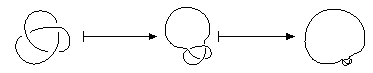
\includegraphics[scale=2]{figures/background/bachelor-unknotting.pdf}
  \caption{Bachelor's unknotting}
\end{figure}
% \noindent Using this, one can argue that arbitrary $K: S^1 \into
% \RR^3$ is isotopic to the unknot.
By shrinking down the region in which the crossings occur, we have
found an isotopy removing all of the crossings of the trefoil. Note,
we could even play it in reverse, and spontaneously generate a trefoil
out of an unknot! Clearly this is undesirable. But we are on the right
track. It turns out the ``correct'' definition will be very similar.
Instead of performing an isotopy on the embeddings themselves, we
perform it on the ambient space. This is known as \emph{ambient
  isotopy}.
\begin{definition}[Ambient Isotopy]
  Let $K_0, K_1$ be knots. Then we say $K_0$ is \emph{ambient
    isotopic} or \emph{equivalent} to $K_1$ iff there exists a map $H
  : [0,1] \times \RR^3 \to \RR^3$ such that
  \begin{enumerate}
    \item For all $\mb x \in \RR^3$, $t \in [0,1]$, the map $H_t(\mb x)
      = H(\mb x, t)$ is a homeomorphism,
    \item For all $s \in S^1$, $H(K_0(s), 0) = K_0(s)$ and
      $H(K_0(s),1) = K_1(s)$, and
    \item $H$ is continuous. \qedhere
  \end{enumerate}
\end{definition}
% \noindent Note the similarity to the definition of isotopy when we
% take $X = Y = \RR^3$.
This turns out to be the ``correct'' notion of equivalence, and with
it, we can begin to partition our knots into equivalence classes.
However, it can often be unwieldy to work with ambient isotopies
directly, as topological embeddings can get quite messy. As such we
often restrict ourselves to a family of knots where ambient isotopy
can be characterized by the \emph{Reidemeister moves}, which affords
us a more combinatorial approach to equivalence. This nice family is
known as the collection of \emph{tame knots}, which are defined in
terms of the even simpler \emph{polygonal knots}. A more careful look
at the definitions of tameness will be given in
\cref{chap:tame-and-wild-knots}.

\section{Tame and Polygonal Knots}\label{sec:polygonal-knots}
% \chapter{Polygonal Knots}\label{chap:polygonal-knots}
In this section, we will (very briefly) examine the ``simplest''
possible knots, \emph{polygonal knots}. If the reader would like a
deeper examination of the topic, they are encouraged to take a look at
\cite{burde2003knots} and \cite{Crowell1963}.

Polygonal knots form the backbone for modern combinatorial knot
theory. The idea is that since they are formed out of finite unions of
straight line segments, they can be studied combinatorially, which
makes them nice. What's a little less obvious is that we can actually
extend some of the resulting ideas to \emph{any} knot ambient isotopic
to a polygonal knot. Indeed, essential results such as
\emph{Reidemeister's Theorem} rely on our knots of interest being
ambient isotopic to polygonal knots.
\begin{definition}[Polygonal Knot]
  A \emph{polygonal knot} $\msf K : S^1 \to \RR^3$ is a knot comprised
  of a finite union of straight line segments.\footnote{Note that we
    will also try to use the \emph{sans-serif} font to distinguish
    polygonal knots from their topological counterparts, since
    sans-serif letters are straight and angular.}
\end{definition}
\begin{figure}[H]
  \centering
  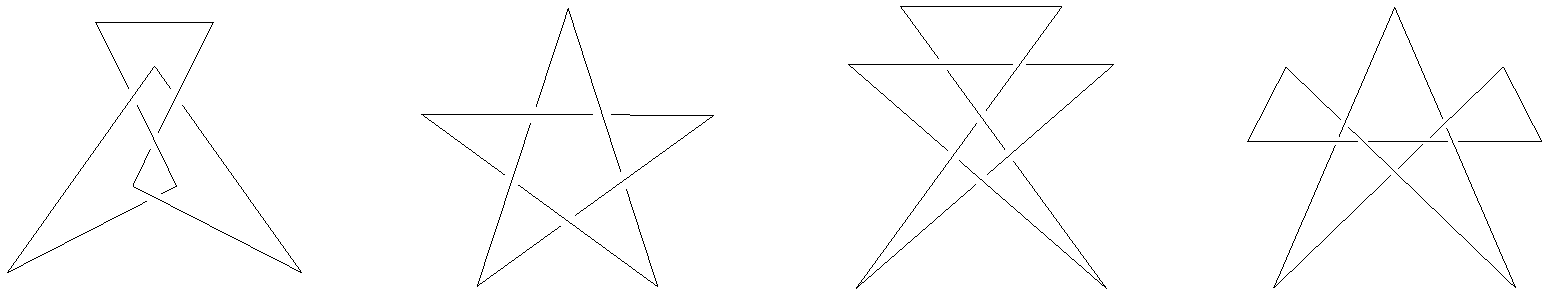
\includegraphics[width=\linewidth]{figures/polygonal-knots/ex-polyknots.pdf}
  \caption{Examples of some polygonal knots}
\end{figure}
It might be helpful to think of polygonal knots in terms of finite
sequences of vertices. This really hammers home the idea that
polygonal knots can be encoded with finite information.
\begin{example}
  We would write the following knot as $\msf{K} = \pn{\msf{v_1, v_2,
      v_3, v_4, v_5, v_6, v_7}}$, where each $\msf{v_i} \in \RR^3$.
  \begin{figure}[H]
    \centering
    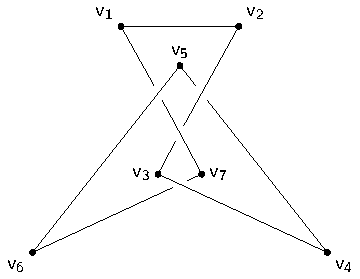
\includegraphics{figures/polygonal-knots/4-1-labeled.pdf}
    \caption[Labeled polygonal $\msf{(4,1)}$]{Polygonal $\msf{(4,1)}$
      knot with vertices labeled} \qedhere
  \end{figure}
\end{example}
The promised combinatorial niceness comes from the following theorem:
\begin{theorem}\label{thm:polygonal-ambient-isotopy}
  Let $\msf K_0, \msf K_1 : S^1 \into \RR^3$ be polygonal knots. Then
  $\msf K_0 \cong \msf K_1$ iff there exists an ambient isotopy $\msf
  F : [0,1] \times \RR^3 \to \RR^3$ with $\msf F(1, \msf K_0) = \msf
  K_1$ that can be realized entirely through a finite sequence of the
  two \emph{elementary moves} (note, in the below, the dashed lines
  are draw somewhat arbitrarily --- we don't really care what the knot
  looks like away from our local picture):
  \begin{enumerate}[label=\arabic*)]
    \item Subdivision:
      \begin{figure}[H]
        \centering
        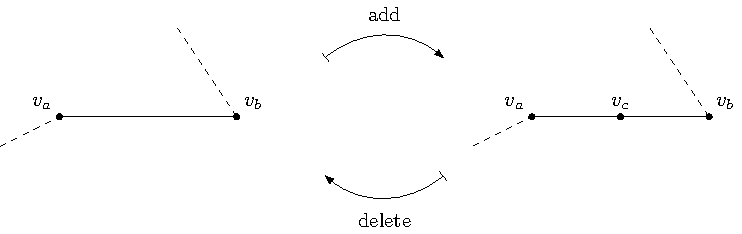
\includegraphics[scale=.85]{figures/fundamentals/el-move-1.pdf}
        \caption[Elementary move 1]{Elementary move 1: adding or
          deleting a vertex}
      \end{figure}
    \item Kinking (note, we require that no line segment passes
      through the triangle in $\RR^3$ with vertices $v_a, v_b, v_c$):
      \begin{figure}[H]
        \centering
        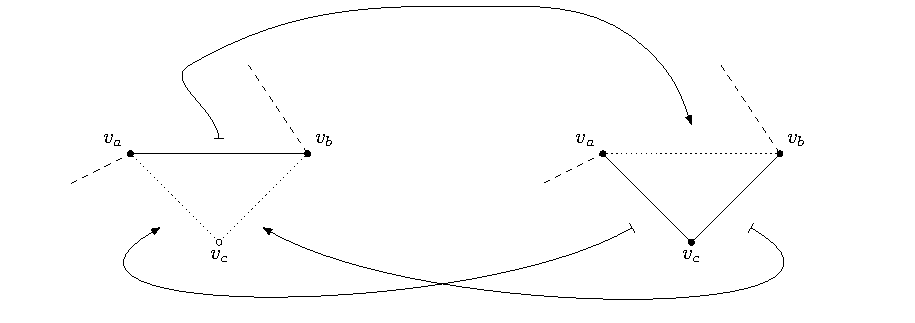
\includegraphics[scale=.85]{figures/fundamentals/el-move-2.pdf}
        \caption[Elementary move 2]{Elementary move 2: swapping edges
          on a triangle}
      \end{figure}
  \end{enumerate}
\end{theorem}
\begin{remark}
  It's worth emphasizing that although we've drawn the moves above to
  appear planar, they're really happening in $\RR^3$. So we
  \emph{could} have all sorts of things happening above or below our
  region of interest. We just need to require that there are no
  obstacles in performing the kink move.
\end{remark}
We will not offer a proof of the theorem, since working with ambient
isotopy directly turns out to be somewhat of a headache, and the proof
won't be terribly informative for the contexts we \emph{do} interact
with ambient isotopy in later on. The point is just to illustrate how
simple ambient isotopy is for polygonal knots.

We now define \emph{tame knots} from polygonal knots.
\begin{definition}[Tame Knot]
  Let $K : S^1 \into \RR^3$ be a knot. Suppose that there exists a
  polygonal knot $\msf K : S^1 \into \RR^3$ such that $K \cong \msf
  K$. Then we say \emph{$K$ is a tame knot}.
\end{definition}
We call knots that are not tame \emph{wild} knots. Little is known
about wild knots; they are the focus of \cref{part:wild-knots}.
\begin{figure}[H]
  \begin{minipage}{.49\linewidth}
    \begin{figure}[H]
      \centering
      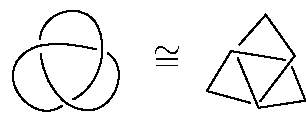
\includegraphics{figures/background/polygonal-knot.pdf}
      \caption{Example of a tame knot}
    \end{figure}
  \end{minipage}
  \begin{minipage}{.49\linewidth}
    \vspace{1.25em}
    \begin{figure}[H]
      \centering
      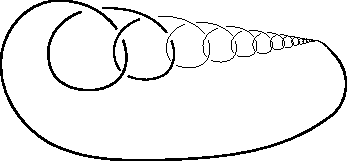
\includegraphics[scale=.6]{figures/background/wild-knot-example.pdf}
      \caption{Example of a wild knot (the loops repeat infinitely)}
    \end{figure}
  \end{minipage}
\end{figure}
The next step in constructing our theory is to state Reidemeister's
theorem for tame knots, which will allow us to turn the 3D moves in
\cref{thm:polygonal-ambient-isotopy} into purely 2D moves on diagrams.
In order for this to work, we need our diagrams to give us enough
information to reconstruct everything that's going on in $3$D up to
ambient isotopy.
% This is the focus of the next section is on understanding knot
% diagrams and why they're special.
% Now Reidemeister's theorem follows from


 % However,
% \cref{thm:all-ambient-isotopic-in-r2} from \cref{part:wild-knots}



% In building up our theory of knots, it will be useful to employ two
% distinct equivalence relations on polygonal knots. The first (known as
% \emph{planar isotopy}) is finer than the second (which I will refer to
% as \emph{polygonal ambient isotopy}).\footnote{Here, ``finer'' means
%   that planar isotopy breaks polygonal knots into more equivalence
%   classes than polygonal ambient isotopy does. This does not imply
%   that planar isotopy is the more ``natural'' choice for definign
%   equivalence of polygonal knots; as we will see, polygonal ambient
%   isotopy corresponds more directly with the general definition of
%   ambient isotopy that we gave before.} However, this granularity
% comes at a price --- planar isotopy doesn't allow us to change any
% crossings. As such, we can't say the following knots are equivalent by
% planar isotopy:
% \begin{figure}[H]
%   \centering
%   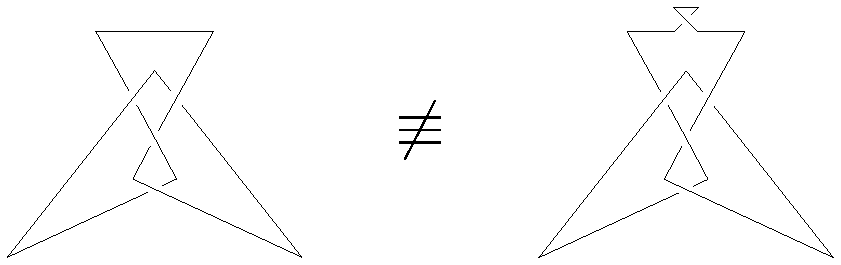
\includegraphics[scale=.5]{figures/polygonal-knots/non-planar-isotopic-example.pdf}
%   \caption[Ambient isotopic but not planar isotopic]{Two polygonal
%     knots that are not planar isotopic}
% \end{figure}
% {\color{red} if choosing to use $\equiv$ exclusively for planar
%   isotopy, add this to the preface}

% {\color{red} come back and talk about polygonal knots vs polygonal
%   knot diagrams}

% {\color{red} come back and change the word ``involved'' to
%   ``incident'' or something and define that elsewhere}

% Ok, now the definitions.
% \subsection{Elementary Moves}
% Elementary moves are the building blocks for {\color{red} a bunch of
%   stuff. Let's define them.}
% \begin{definition}[Elementary Moves]
%   Let $\msf{K} = \pn{\msf{v_1, \ldots, v_n}}$ be a polygonal knot.
%   Then an elementary is an insertion/deletion of a vertex in $\msf K$
%   as follows:
%   \begin{enumerate}
%     \item Suppose {\color{red} return to this}
%     \item
%   \end{enumerate}
% \end{definition}

% \subsection{Planar Isotopy}
% Planar isotopy is based on the idea of a \emph{planar move}. These
% are special elementary moves that
% \begin{definition}[Planar Moves]\label{def:planarmoves}
%   Let $\msf{K = \pn{v_1,\ldots, v_n}}$ be a polygonal knot. A
%   \emph{planar move} on $\msf K$ corresponds to the insertion or
%   deletion of a vertex in $\msf{K}$ per one of the following cases
%   (see {\color{red} insert ref here} for diagrams):
%   \begin{enumerate}
%     \item Insertion rules: Let $\msf{v_i, v_{i+1}}$ be sequential
%       vertices in $\msf{K}$ and let $\msf{v_{new}} \in \RR^3$.
%       Suppose we have one of the following cases:
%       \begin{enumerate}
%         \item Subdivision: Suppose that $\msf{v_{new}}$ is on the line
%           segment connecting $\msf{v_i, v_{i+1}}$.
%         \item Kink on a free segment: Suppose that the line segment
%           $(\msf{v_i}, \msf{v_{i+1}})$ is not involved in any
%           crossings in $\msf{K}$ and the line segments defined by
%           $\msf{\pn{v_i, v_{new}}}$ and $\msf{\pn{v_{new}, v_{i+1}}}$
%           also aren't involved in any crossings.
%         \item Kink on a crossing
%           segment:\footnote{\label{foot:nonredundant} This is not
%             redundant with the subdivision rule. See {\color{red}
%               Insert ref to remark here} for explanation.} Suppose
%           that the line segment $\pn{\msf{v_i, v_{i+1}}}$ is involved
%           in exactly one crossing in $\msf{K}$. Denote the crossed
%           strand by $\pn{\msf{v_j, v_{j+1}}}$ and suppose that
%           \emph{exactly one} of $\pn{\msf{v_i, v_{new}}}$ or
%           $\pn{\msf{v_{new}, v_{i+1}}}$ crosses $\pn{\msf{v_i,
%               v_{i+1}}}$. Denote this segment by $\msf{e_{cross}}$ and
%           the other by $\msf{e_{free}}$. Finally, suppose that
%           $\msf{e_{cross}}$ crosses over/under $\pn{\msf{v_j,
%               v_{j+1}}}$ iff $\pn{\msf{v_i, v_{i+1}}}$ does, and that
%           $\msf{e_{free}}$ is not involved in any crossings.
%       \end{enumerate}
%       Then in any of these cases, the insertion
%       \[
%         \msf{\pn{v_1, \ldots, v_i, v_{i+1}, \ldots, v_n}} \mapsto
%         \msf{\pn{v_1, \ldots, v_i, {\color{blue} v_{new}}, v_{i+1},
%             \ldots, v_n}}
%       \]
%       is a planar move.
%     \item Deletion rules: These correspond to undoing the moves above.
%       Let $\msf{v_{i-1}, v_{i}, v_{i+1}}$ be sequential vertices in
%       $\msf{K}$; here $\msf{v_i}$ corresponds to $\msf{v_{new}}$
%       above. Suppose that we have one of the following cases:
%       \begin{enumerate}
%         \item Subdivision: Suppose that $\msf{v_i}$ is on the line
%           segment $\pn{\msf{v_{i-1}, v_{i+1}}}$.
%         \item Kink on a free segment: Suppose that none of the line
%           segments defined by $\msf{\pn{v_{i-1}, v_i}, \pn{v_i,
%               v_{i+1}}}$, and $\msf{\pn{v_{i-1}, v_{i+1}}}$ are
%           involved in crossings.
%         \item Kink on a crossing segment: Suppose that exactly one of
%           $\pn{\msf{v_{i-1},v_i}}$ and $\pn{\msf{v_i, v_{i+1}}}$ is
%           involved in a single crossing, and that the other is
%           involved in no crossings. Denote the crossed strand by
%           $\msf{e_{cross}}$, and suppose that $\msf{v_{i-1}, v_{i+1}}$
%           crosses $\msf{e_{cross}}$ in the same way (over if over,
%           under if under).
%       \end{enumerate}
%       Then in any of these cases case, the deletion
%       \[
%         \msf{\pn{v_1, \ldots, v_{i-1}, {\color{blue} v_i},
%             v_{i+1}, \ldots, v_n}} \mapsto \msf{\pn{v_1, \ldots,
%             v_{i-1}, v_{i+1}, \ldots, v_n}}
%       \]
%       is a planar move.
%   \end{enumerate}
% \end{definition}
% \begin{remark}
%   As noted in \cref{foot:nonredundant}, the \emph{subdivision} and
%   \emph{kink on a crossing segment} moves are not redundant. The
%   reason is that \emph{subdivision} is allowed even when multiple
%   strands cross $\pn{\msf{v_i, v_{i+1}}}$, whereas \emph{kink on a
%     crossing segment} doesn't. {\color{red} Is it worth keeping these
%     definitions separate, or should I try and roll them together?}
% \end{remark}

% \begin{figure}[H]
%   \centering
%   \includegraphics[draft]{figures/polygonal-knots/planar-moves.pdf}
%   \caption{Planar moves}
% \end{figure}

% \begin{proposition}
%   Finite sequences of planar moves can never add or remove crossings
%   in a diagram for $\msf{K}$.
% \end{proposition}
% \begin{proof}
%   Each of the three moves defined in \cref{def:planmoves} preserve the
%   number of crossings in $\msf{K}$. The finiteness condition prevents
%   us from getting situations like the following:
%   \begin{figure}[H]
%     \centering
%     \includegraphics[draft]{figures/polygonal-knots/losing-a-crossing.pdf}
%     \caption{Sequence losing a crossing in the limit}
%   \end{figure}
% \end{proof}

% % \begin{proposition}
% %   This implies moves that change \emph{multiple} crossings are ok. But
% %   we will only consider single crossings
% % \end{proposition}
% \subsection{Polygonal Ambient Isotopy and Reidemeister's Theorem}
% We want to develop an equivalence relation that \emph{does} allow us
% to modify crossings. This will be furnished by \emph{polygonal ambient
%   isotopy}, which mirrors the definition of \emph{ambient isotopy} for
% general topological knots.

% Recall that we defined a general ambient isotopy to be a continuous
% deformation of the ambient space that restricts to a homotopy
% \emph{through} knots, starting with $K_0$ and ending with $K_1$.
% {\color{red} come back and revise; this isn't quite right.} We'll
% define polygonal ambient isotopy similarly, only now we require our
% function to restrict to a homotopy through \emph{polygonal knots}.
% \begin{definition}[Equivalence of Polygonal Knots]
%   Let $\msf{K_1}$, $\msf{K_2} : S^1 \to (X, \ms T)$ be polygonal
%   knots. Then we say $\msf{K_1, K_2}$ are \emph{equivalent} or
%   \emph{polygonally ambient isotopic} iff there exists an ambient
%   isotopy $\msf F : X \times [0,1] \to X$ such that for each $t \in
%   [0,1]$, $\msf F(\msf{K_1}, t)$ is a polygonal knot.
% \end{definition}
% We want to be able to characterize polygonal ambient isotopy in terms
% of simple moves like those employed in \emph{planar} isotopy. The
% means to do so are furnished by \emph{Reidemeister's Theorem},
% {\color{red} one of the crowning achievements of knot theory during
%   the early 20\textsuperscript{th} century}. Note, {\color{red} talk
%   about how today we actually prove something from which
%   Reidemeister's Theorem follows as a corollary}

% {\color{red} This next lemma tells us that strands of our knots are
%   separated in some sense }
% \begin{lemma}
%   Let $\msf K$ be a polygonal knot. Let $\msf{e_1, e_2}$ be line
%   segments in $\msf K$ that do not share a vertex (note, this implies
%   $\msf{e_1 \neq e_2}$). Then
%   \[
%     \inf_{\substack{\msf{x_1} \in \msf{e_1} \\ \msf{x_2} \in
%         \msf{e_2}}} d(\msf{x_1, x_2}) > 0.
%   \]
% \end{lemma}
% \begin{proof}
%   We have two cases.
%   \begin{enumerate}[label=\arabic*)]
%     \item Suppose $\msf{e_1}$ is parallel to $\msf{e_2}$. Then since
%       $\msf{e_1} \cap \msf{e_2} = \varnothing$, {\color{red}
%         aaaaaaaaaaaaaaaa this means the distnace is constant between
%         them something something use multi calc if you'd like}
%     \item Suppose $\msf{e_1}$ is not parallel to $\msf{e_2}$.
%   \end{enumerate}

%   Suppose not. Then $\forall \varepsilon > 0$, there exist
%   $\msf{x_{1}} \in \msf{e_1}$ and $\msf{x_{2}} \in \msf{e_2}$ such
%   that $d(\msf{x_1}, \msf{x_2}) < \varepsilon$. Now, consider the
%   sequence
%   \[
%     \varepsilon_n = \frac{1}{n} \qquad\qquad \text{for all }n \in \NN,
%   \]
%   and let $\pn{\msf{x_{1,n}}}_{n\in\NN}$,
%   $\pn{\msf{x_{2,n}}}_{n\in\NN}$ be sequences of points in
%   $\msf{e_1,e_2}$ respectively such that for all $n \in \NN$,
%   $d(\msf{x_{1,n}, x_{2,n}}) < \varepsilon_n$. Now, let
%   \[
%     \msf{x_1} = \lim_{n\to\infty} \msf{x_{1,n}}\qquad \text{and}
%     \qquad \msf{x_2} = \lim_{n\to\infty} \msf{x_{2,n}}.
%   \]
%   {\color{red} Wait how do we know these limits exist?}

%   Note, $\msf{e_1, e_2}$ are line segments in $\RR^3$ and are thus
%   closed. It follows that they are complete, so we have $\msf{x_{1},
%     x_2}$. Hence, Now, $\msf{x_1} = \msf{x_2}$
% \end{proof}

% \begin{corollary}\label{cor:elarepolyamb}
%   Elementary moves are polygonal ambient isotopies.
% \end{corollary}
% \begin{proof}
%   {\color{red} Come back and fill in the details. Just do the
%     straight-line homotopy between the edges}
% \end{proof}

% \begin{theorem}

% \end{theorem}


% \begin{theorem}
%   Let $\msf{K_1, K_2}$ be polygonal knots. Then the following are
%   equivalent:
%   \begin{enumerate}
%     \item $\msf{K_1}$ and $\msf{K_2}$ are polygonally ambient
%       isotopic,
%     \item There exists an orientation-preserving homeomorphism $f :
%       \RR^3 \to \RR^3$ such that $f(\msf{K_0}) = \msf{K_1}$.
%     \item $\msf{K_1}$ and $\msf{K_2}$ are related by a finite sequence
%       of elementary moves,
%   \end{enumerate}
% \end{theorem}
% \begin{proof}
%   We base our exposition on the argument given in
%   \cite{burde2003knots}. We first prove $1 \iff 2$ and then prove $2
%   \iff 3$.
%   \begin{enumerate}[label=(\alph*)]
%     \item We want to show $1 \iff 2$.
%       \begin{iffproof}
%         \item Suppose that $\msf{K_1}$, $\msf{K_2}$ are polygonally
%           ambient isotopic by some $F : \RR^3 \times [0,1] \to \RR^3$.
%           {\color{red} Come back and double check whether we really
%             want $X$ here}. Then taking $f = F(\cdot, 1)$ yields the
%           desired orientation-preserving homeomorphism.
%         \item Suppose that there exists an orientation-preserving
%           homeomorphism $f : \RR^3 \to \RR^3$ such that $f(K_0) =
%           K_1$.

%           \textbf{Claim 1:} There exists an ambient isotopy $F : \RR^3
%           \times [0,1] \to \RR^3$ such that
%       \end{iffproof}
%   \end{enumerate}
% \end{proof}

% \begin{proof}~
%   \begin{iffproof}
%     \item This follows from \cref{cor:elarepolyamb}
%     \item Suppose that $\msf{K_1, K_2}$ are polygonally ambient
%       isotopic, denote the polygonal ambient isotopy by $\msf F$.

%       For each $t \in [0,1]$, $\msf{F}(\msf{K_1}, t)$ is a polygonal
%       knot. Thus, at each time $t$,
%       \begin{itemize}
%         \item Our knot is a finite union of straight line segments
%         \item By continuity, $\forall \varepsilon > 0$, there exists a
%           $\delta > 0$ such that things being within delta of each
%           other make the difference less than $\varepsilon$
%         \item Choose $\varepsilon$ to be $1/2$ of the minimizing
%           distance between points on any two of the line segments
%           making up $K_1$ (such a min exists by finitely many line
%           segments condition).
%         \item This gives us the first set of elementary moves.
%         \item
%       \end{itemize}
%   \end{iffproof}
% \end{proof}

% {\color{red} How are elementary moves realized in the Diagrams??????
%   IDK Reidemeister Theorem time }
% \begin{theorem}
%   \color{red} AAAAAAAAAAAAAAAAAAAAAAAAAAAAAAAAAAAAa
% \end{theorem}



% \section{Tame Knots and Regular Diagrams}

% \begin{theorem}
%   Two knots $K_1, K_2$ are ambient isotopic iff their polygonal
%   representations $\msf{K_1, K_2}$ are polygonally isotopic.
% \end{theorem}

% {\color{red} Insert examples here}

% \begin{definition}[Smooth Knots]
%   AAAAAAAAAAAAAAAAAAAAAAAAa
% \end{definition}

% \begin{definition}[Tame Knots]
%   A knot is called \emph{tame} aaaaaaaaaaaaaaaaaaaaaaaaaaaaa
% \end{definition}

% \begin{definition}[Wild Knots]
%   Give the definition
% \end{definition}







% \section{Regular Diagrams and Reidemeister's Theorem}






% {\color{red} Return and make sure this is integrated well at some
%   point}

% We want to study knots (and the knot equivalence problem) from a
% combinatorial perspective. To do so,



% Now, we can partition knots into two important sets
% Now, we can talk about the difference between so-called \emph{tame}
% knots and \emph{wild} knots.
% Loosely speaking, a diagram of a tame
% knot can be encoded with finite amounts of information, while a
% diagram for a wild knot cannot (we'll talk about this more in the
% next section).
% Knots come in two flavors
% : \emph{tame knots} and \emph{wild knots}. Loosely speaking,
% \emph{tame knots} can be approximated by finitely many straight-line
% segments, while \emph{wild knots} cannot (we discuss this in the next
% chapter).\\
% \begin{minipage}{.49\linewidth}
%   \begin{figure}[H]
%     \centering
%     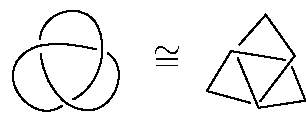
\includegraphics{figures/background/polygonal-knot.pdf}
%     \caption{Example of a tame knot}
%   \end{figure}
% \end{minipage}
% \begin{minipage}{.49\linewidth}
%   \vspace{1.25em}
%   \begin{figure}[H]
%     \centering
%     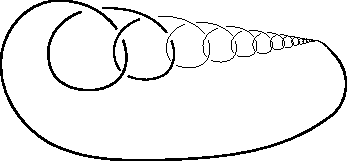
\includegraphics[scale=.6]{figures/background/wild-knot-example.pdf}
%     \caption{Example of a wild knot (the loops repeat infinitely)}
%   \end{figure}
% \end{minipage}\vspace{.5em}
% Currently, we understand tame knots fairly well but know very little
% about wild knots. Much of modern knot theory is built on top of
% \emph{Reidemeister's Theorem}, which offers us a way of understanding
% tame knots by applying simple manipulations to their diagrams. For
% this theorem to hold, though, we need our diagrams to be on their best
% behavior. In the next section we examine what this
% means.


\section{Knot Diagrams}\label{sec:KnotDiags}
When first learning about functions $f : \RR \to \RR$ (e.g., in a
Calculus I course), we are often taught to think of \emph{functions}
and \emph{graphs of functions} interchangeably. For instance, if we
were given
\[
  f(x) = -\frac{x^2}{4} + 2x,
\]
we'd probably imagine a picture similar to the following:
\begin{figure}[H]
  \centering
  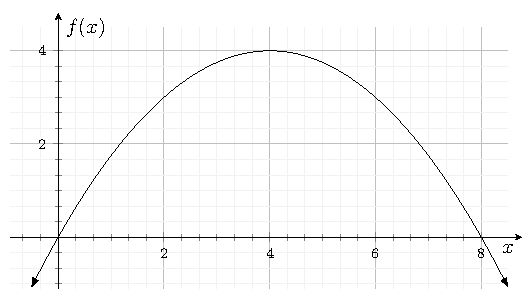
\includegraphics{figures/background/parabola.pdf}
  \caption{Plot of $f(x) = -\frac{x^2}{4} + 2x$}
  \label{fig:plotoffunc}
\end{figure}
\noindent Hence, we might be mystified to see a definition like the
following in an Analysis I book.
\begin{definition}[Graph of a Function]
  Let $f : X \to Y$. The \emph{graph} of $f$ is defined to be
  \[
    G(f) = \set{(x, f(x)) \MID x \in X}.
  \]
  Note $G(f) \subset X \times Y$, and when $X = Y = \RR$, we often
  represent $G(f)$ visually by plots like in \cref{fig:plotoffunc}.
\end{definition}
This is confusing. Why have we made this extra definition? Does its
presence mean there's a flaw in thinking of a function and its graph
interchangeably?

% {\color{red} \Huge come back and redo this part}

Well, sort of, but they don't really cause problems for $f : \RR \to
\RR$. First, note that in modern set theory, the definition of ``Graph
of a Function'' we gave above is actually how \emph{functions
  themselves} are defined formally. Nonetheless, there are some
caveats, e.g.\
\begin{itemize}
  \item Our picture here doesn't actually include the full domain of
    the function, because our drawing space is finite.
  % \item Often, we like to think of functions as \emph{maps}. In this
  %   case, it can be important to define the \emph{domain} and
  %   \emph{codomain} of the function explicitly. Our set-theoretic
  %   definition for $G(f)$ does not include this information (in
  %   particular, we don't explicitly know what the codomain is).
    % {\color{red} come back and rework this}
  \item For multivariable functions, e.g. $f : \RR^2 \to \RR$, it is
    often no longer possible to give an injective 2D representation of
    $G(f)$ without making some concessions. In particular, we are
    constrained to represent $G(f)$ on a 2D canvas, so we can't just
    plot a point at every $(x,y,z)$ pair.
\end{itemize}
We'll focus on the latter for today. How do we represent 3D objects in
2D? Often, we try to find clever ways of including extra information
in our diagrammatic representations such that we can recover some of
the information we lose in projection. In the particular case of $f :
\RR^2 \to \RR$, we have various tools at our disposal, such as making
use of \emph{color}, \emph{grid lines} and
\emph{contours}.\\
\begin{minipage}{.49\linewidth}
  \begin{figure}[H]
    \centering
    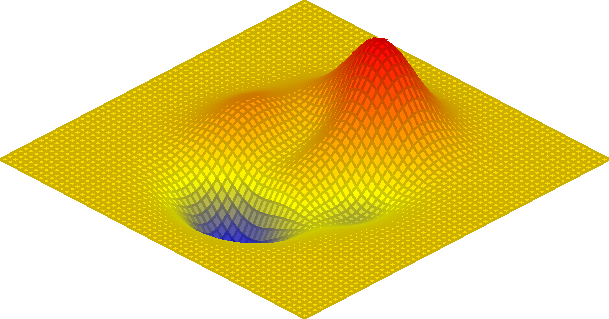
\includegraphics[scale=.57]{figures/background/surface.pdf}
    \caption{A surface}
  \end{figure}
\end{minipage}
\begin{minipage}{.49\linewidth}
  \begin{figure}[H]
    \centering
    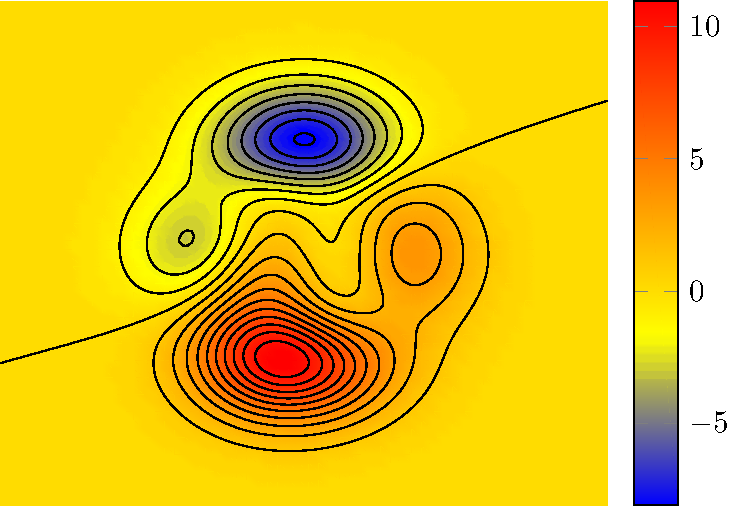
\includegraphics[scale=.37]{figures/background/surface-contour.pdf}
    \caption{Contour plot of the same surface}
  \end{figure}
\end{minipage}\\
Using these tools, we can create 2D representations from which we can
(more or less) reconstruct the $3$D picture we started with. We will
employ a similar idea in dealing with knots, although this turns out
to be a bit of a delicate matter. In particular, because we want to
make diagrams our fundamental object of study, in order to maintain
rigor we must be \emph{very exacting} in understanding \emph{what} our
diagrams represent, and \emph{how} we can pull that back to a result
about our actual knot in $3$D. \hfill $\lozenge$

We motivate this with the following examples.
\subsection{What makes a ``helpful'' knot diagram}

As we have seen, it is often useful to represent knots by 2D diagrams.
However, not all diagrams are equivalently helpful. For instance, if
we were to ``line up'' all the crossings of the $(7,2)$ knot like so,
\begin{figure}[H]
  \centering
  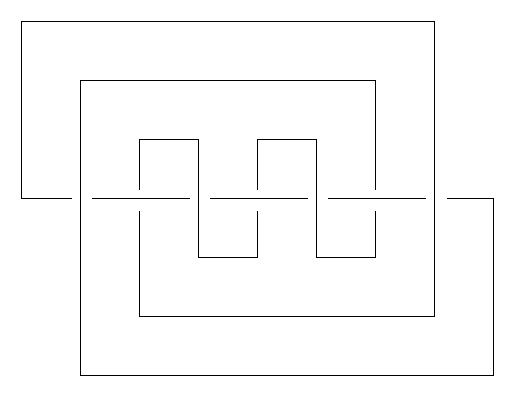
\includegraphics[scale=.5]{figures/background/rl_7_2.pdf}
  \caption{$(7,2)$ with crossings lined up}
  \label{fig:rl72}
\end{figure}
then if we were to look along the following axis,
\begin{figure}[H]
  \centering
  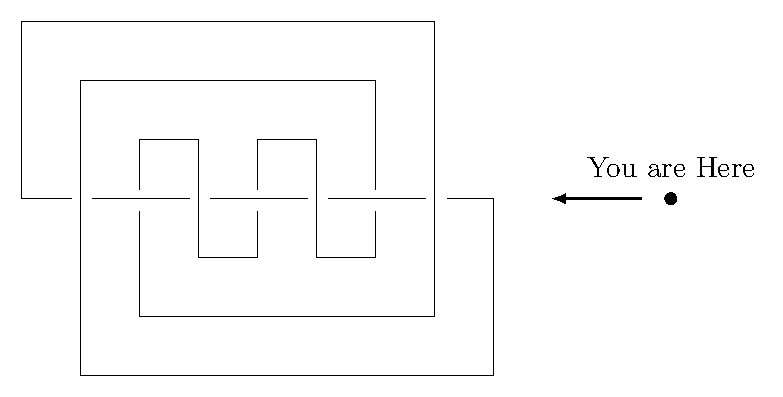
\includegraphics[scale=.6]{figures/background/rl_7_2_view.pdf}
  \caption{New perspective}
\end{figure}
we might end up seeing something like this:
\begin{figure}[H]
  \centering
  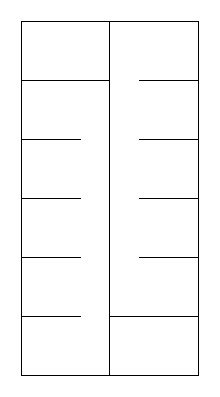
\includegraphics[width=2cm]{figures/background/rl_7_2_side.pdf}
  \caption{Unhelpful sideways view}
  \label{fig:unhelpfulside}
\end{figure}
\noindent which is hardly helpful.\footnote{Note, we say ``might''
  because there are multiple possible 3D realizations that could yield
  \cref{fig:rl72} in a 2D projection. But at least one of those would
  look like \cref{fig:unhelpfulside}.} Hence, we will place some
restrictions on what exactly we are allowed to refer to as a
\emph{knot diagram}. The standard set of rules here are for what are
known as \emph{regular diagrams}.
% First, we'll begin with the definition of a
% \emph{regular knot diagram}, and then prove that there exists a
% regular diagram for $K$ iff $K$ is tame.
\begin{definition}[Regular Knot Diagram]
  Let $K$ be a knot, and let $\pi : \RR^3 \to \RR^2$ be a projection
  onto a $2$-dimensional subspace of $\RR^3$. Then we say $D = \pi
  \circ K(S^1)$ is a \emph{diagram} for $K$ iff $D$ satisfies the
  following conditions:
  \begin{enumerate}[label=\arabic*)]
    \item $D$ is injective at all but finitely many points
      $\set{y_i}_{i=1}^n \in \RR^2$, called \emph{crossings}.
    \item For each of these $y_i$, there exist exactly two $x \in S^1$
      such that $D(x) = y_i$.
    \item Each crossing ``looks like an $X$.'' Formally, there exists
      $\varepsilon > 0$ such that $B_\varepsilon(y_i) \cap D(S^1)$ is
      homeomorphic to $\set{(x,y) \MID x = 0 \text{ or } y = 0}$.
    \item The diagram contains some information by which we can
      recover which strand was ``on top'' at each crossing.
  \end{enumerate}
\end{definition}
\begin{note}
  If $K$ is oriented, we also require the diagram to include
  information that allows us to recover the orientation.
\end{note}
We interpret these properties as follows. Condition (1) requires
that strands only cross at \emph{single points} in our diagrams (not
entire line segments).
\begin{figure}[H]
  \centering
  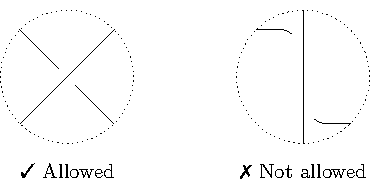
\includegraphics{figures/background/point_cross.pdf}
\end{figure}
Condition (2) requires that we can't have multiple strands crossing at
the same point: % {\color{red} should these conditions be hyperref'ed}
\begin{figure}[H]
  \centering
  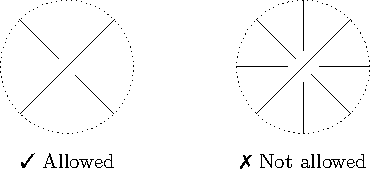
\includegraphics{figures/background/single_cross.pdf}
\end{figure}
Condition (3) precludes situations like the following:
\begin{figure}[H]
  \centering
  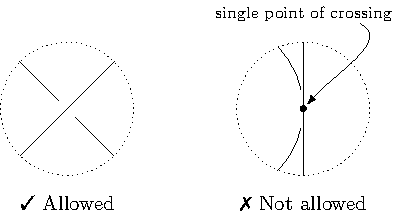
\includegraphics{figures/background/x_cross.pdf}
\end{figure}
\noindent that is, we don't allow crossings to take the form of
``tangencies;'' both of the strands that come in must leave on
opposite sides. Finally, condition (4) actually refers to a convention
that we have been employing tacitly all along; namely \emph{breaks} in
the diagram represent places were crossings occur, and the broken
strand is understood to be going ``underneath'' the unbroken strand.
\begin{figure}[H]
  \begin{center}
    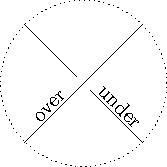
\includegraphics[width=2.5cm]{figures/background/uo_cross.pdf}
  \end{center}
  \caption{Breaks tell us which strand is on top}
\end{figure}
Now, we have the following important theorem:
\begin{theorem}
  Let $K : S^1 \into \RR^3$ be a knot. Then $K$ is tame iff there
  exists a regular diagram $D$ of $K$.
\end{theorem}
\begin{proof}
  Left as an exercise. \emph{Hint:} For the forward direction, first,
  prove a lemma showing that for conditions (2), (3), and (4), we can
  deform the space ever so slightly to fix all of our issues. For
  condition (1), do the same and then use the finite polygonal
  representation to get injectivity at all but finitely many points.

  There are a number of ways to do the back direction. Use the diagram
  to get your polygonal representation.
\end{proof}
Later, it will be helpful to draw diagrams of \emph{wild} knots as
well as tame knots, hence we make the definition below. To the best of
my knowledge, this is not something that has been treated before.
\begin{definition}[Regular Diagrams for Wild Knots]
  Identical to the definition for a \emph{regular knot diagram},
  except we allow injectivity to fail at a countable collection of
  points.
\end{definition}
In general, all knots and their diagrams are assumed to be \emph{tame}
unless otherwise stated.
\begin{remark}
  At this point, let's take some time again to highlight the
  difference between a \emph{knot} and a \emph{regular diagram}. A
  \emph{knot} is an abstract function going from $S^1$ to $\RR^3$,
  while a \emph{regular diagram} is a function going $S^1$ to $\RR^2$.
  In the section above, we defined knot diagram $D$ in terms of
  composing a particular projection $\pi$ with a knot $K$. However, we
  can also think of $D$ as an abstract function in its own right. This
  gives us the following commutative diagram:
  \begin{figure}[H]
    \centering
    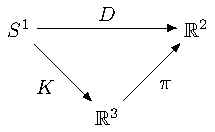
\includegraphics{figures/background/D_comm_diag.pdf}
    \caption{Relationships between $D, K$, and $\pi$}
  \end{figure}
  \noindent It's worth nothing that this factorization is not unique!
  In particular, we can have many different $K,\pi$ pairs that give us
  the same $D$:
  \begin{figure}[H]
    \centering
    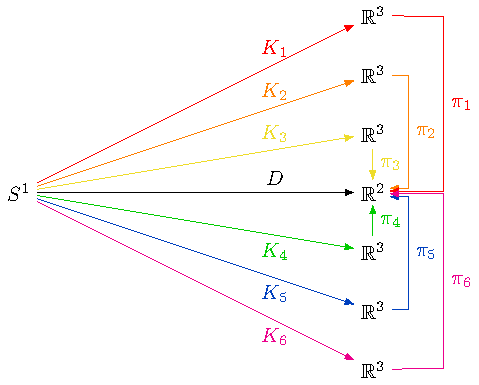
\includegraphics{figures/background/same_D_diff_factors.pdf}
    \caption{Taste the rainbow!}
  \end{figure}
  I feel like having multiple copies of $\RR^3$ might be an abuse of
  commutative diagram notation (I'm sorry to any Category Theory
  enthusiasts out there), but hopefully it gets the point across.
  Anyways, in sort of dual vein, different projections $\pi$ can take
  the same knot $K$ to many \emph{different} diagrams.
  \begin{figure}[H]
    \centering
    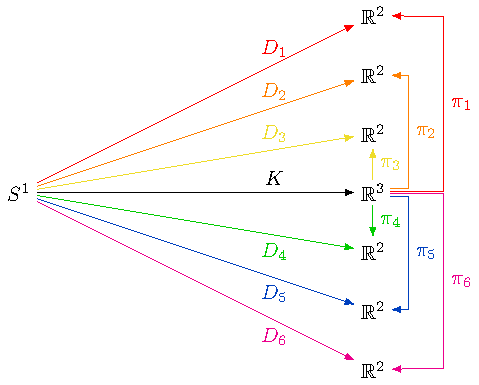
\includegraphics{figures/background/multiD_comm_diag.pdf}
    \caption{Another colorful diagram}
  \end{figure}
\end{remark}
Both of these properties are undesirable. In order to use diagrams to
study knots, we must figure out a way to ensure that they ``contain
the same information'' in some sense. In particular, we want to define
an \emph{equivalence} relation on the category of regular diagrams
such that equivalence classes of diagrams correspond exactly to
equivalence classes of knots under ambient isotopy. This is what
\emph{Reidemeister's Theorem} allows.
\begin{theorem}[Reidemeister, 1927]
  Let $K_0, K_1 : S^1\into \RR^3$ be tame knots, and let $D_0, D_1$ be
  regular diagrams for $K_0, K_1$. Then $K_0 \cong K_1$ iff $D_0$ can
  be turned into $D_1$ by applying a finite sequence of the following
  moves:
  \begin{figure}[H]
    \centering
    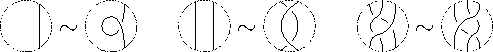
\includegraphics[scale=1.5]{figures/intro/rmoves.pdf}
  \end{figure}
  \noindent together with ``planar isotopy:''
  \[
    \preri
    \ \raisebox{.25em}{$\mathlarger{\mathlarger{\sim}}$}\ \rzero
  \]
  i.e., we can arbitrarily reshape a strand in a neighborhood provided
  we don't change the endpoints or the crossing information.
\end{theorem}
Note, if we can locally straighten out $K_0, K_1$ to look like
polygonal knots, the theorem follows as a straightforward corollary to
\cref{thm:polygonal-ambient-isotopy}. This is the point that most
proofs of Reidemeister's theorem start from (see
\cite{prasolov1997knots}, for instance). However, getting there is not
entirely trivial, as topological embeddings can be extremely
poorly-behaved. For instance, our knot could look like the
Weierstrass\footnote{Pronunciation guide: \ipa{"vaI5StKa:s}} function
from the side, but a plain straight line from the top.
\begin{figure}[H]
  \centering
  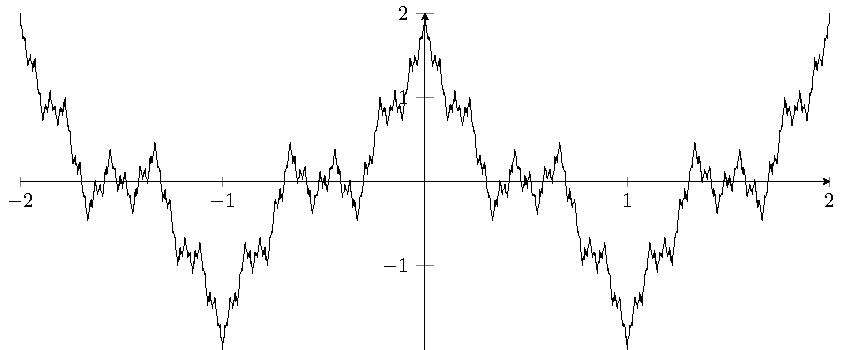
\includegraphics[scale=.9]{figures/fundamentals/weirstrass.pdf}
  \caption{Side-view: Weierstrass function}
\end{figure}
\begin{figure}[H]
  \centering
  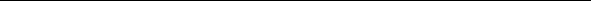
\includegraphics[scale=1.3]{figures/fundamentals/straight-line.pdf}
  \caption{Top-down-view: Just a line}
\end{figure}
We address this rigorously in \cref{part:wild-knots} once we have the
machinery to discuss lifting ambient isotopies from $\RR^2$ to
$\RR^3$, but until then, we hope the high-level ideas have been
communicated to the reader satisfactorily.%  The ensuing chapters will
% be much more technically-focused.

\section{Orientation}
The final concept we'll add to our knots is \emph{orientation}. Note,
if we pick an arbitrary point $s \in S^1$, there are two options for
how to transverse the curve before ending up back where we started. We
call these \emph{orientations}.
\begin{figure}[H]
  \centering
  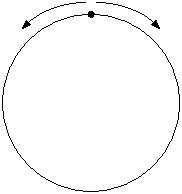
\includegraphics{figures/fundamentals/orientation-on-s1.pdf}
  \caption{The two possible choices of orientation on $S^1$}
\end{figure}
We can think of the orientation as giving us a canonical ordering of
the elements of $S^1$.\footnote{The interested reader should read more
  about \emph{cyclic orders}. An interesting note is that unlike the
  traditional $<$ relation we're used to in $\RR$, cyclic orders are
  not binary relations. It doesn't really make sense to say ``$s_1 <
  s_2$'' in $S^1$, since if we simply continue out from $s_2$ far
  enough we'll get back to $s_1$, so it would seem $s_2 < s_1$ as
  well. The solution is to employ a \emph{ternary} relation. That is,
  we define an order-like relation by saying $s_1 < s_2 < s_3$ iff we
  encounter $s_1$, $s_2$, $s_3$ sequentially while traversing $S^1$ in
  some direction, and $s_2$ and $s_3$ occur before we see $s_1$
  again.} A choice of orientation on $S^1$ similarly induces an
orientation on our knots, which we denote by arrows in the diagrams.
\begin{figure}[H]
  \centering
  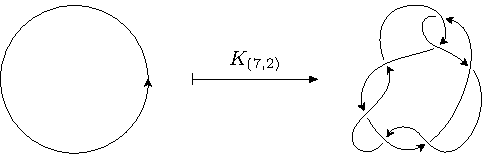
\includegraphics{figures/fundamentals/oriented-72.pdf}
  \caption{An oriented $(7,2)$}
\end{figure}
An interesting consequence of this fact is that crossings are now
chiral, coming in two non-rotationally-equivalent flavors. We refer to
them as \emph{positive} and \emph{negative} respectively, according to
the right hand rule.\footnote{Point your index finger along the
  overstrand, and middle finger along the understrand. If your thumb
  points up, the crossing is positive, otherwise it's negative.} This
is in contrast to the case with unoriented knots, where all crossings
are rotationally equivalent.
\begin{figure}[H]
  \def\figdir{figures/fundamentals/crossings}
  \centering
  \begin{subfigure}{.24\textwidth}
    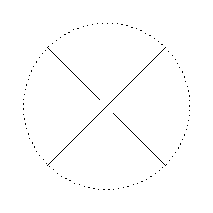
\includegraphics[scale=.65]{\figdir/uo-1.pdf}
  \end{subfigure}
  \begin{subfigure}{.24\textwidth}
    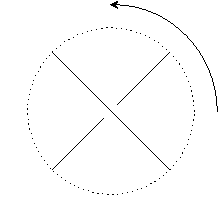
\includegraphics[scale=.65]{\figdir/uo-2.pdf}
  \end{subfigure}
  \begin{subfigure}{.24\textwidth}
    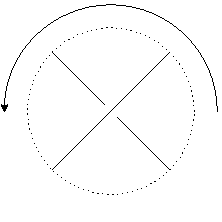
\includegraphics[scale=.65]{\figdir/uo-3.pdf}
  \end{subfigure}
  \begin{subfigure}{.24\textwidth}
    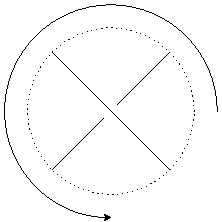
\includegraphics[scale=.65]{\figdir/uo-4.pdf}
  \end{subfigure}
  \caption{Rotating an unoriented crossing $3\times$}
\end{figure}
\begin{figure}[H]
  \def\figdir{figures/fundamentals/crossings}
  \centering
  \begin{subfigure}{.24\textwidth}
    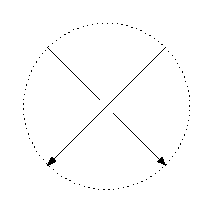
\includegraphics[scale=.65]{\figdir/o1-1.pdf}
  \end{subfigure}
  \begin{subfigure}{.24\textwidth}
    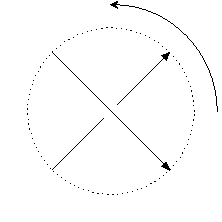
\includegraphics[scale=.65]{\figdir/o1-2.pdf}
  \end{subfigure}
  \begin{subfigure}{.24\textwidth}
    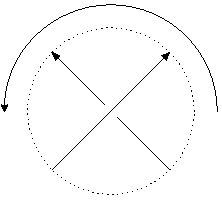
\includegraphics[scale=.65]{\figdir/o1-3.pdf}
  \end{subfigure}
  \begin{subfigure}{.24\textwidth}
    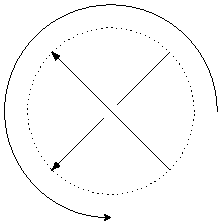
\includegraphics[scale=.65]{\figdir/o1-4.pdf}
  \end{subfigure}
  \caption{Rotating a positive crossing $3\times$}
\end{figure}
\begin{figure}[H]
  \def\figdir{figures/fundamentals/crossings}
  \centering
  \begin{subfigure}{.24\textwidth}
    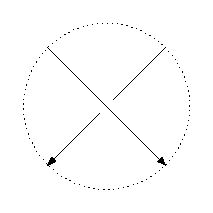
\includegraphics[scale=.65]{\figdir/o2-1.pdf}
  \end{subfigure}
  \begin{subfigure}{.24\textwidth}
    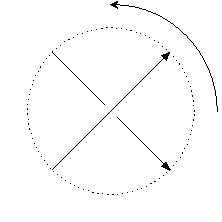
\includegraphics[scale=.65]{\figdir/o2-2.pdf}
  \end{subfigure}
  \begin{subfigure}{.24\textwidth}
    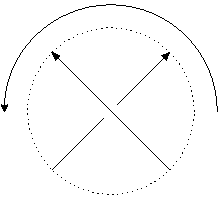
\includegraphics[scale=.65]{\figdir/o2-3.pdf}
  \end{subfigure}
  \begin{subfigure}{.24\textwidth}
    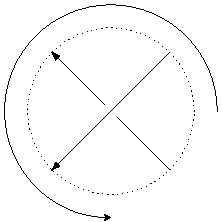
\includegraphics[scale=.65]{\figdir/o2-4.pdf}
  \end{subfigure}
  \caption{Rotating a negative crossing $3\times$}
\end{figure}
As one can see, there is no way to convert a positive crossing to a
negative crossing without performing a reflection on the dotted
neighborhood.

Orientation is important because it's necessary for making certain
operations well-defined. An example is the \emph{connected sum}, which
we define in loose terms below.
\begin{definition}[Connected Sum]
  Let $K_0, K_1$ be oriented knots, with associated diagrams $D_0,
  D_1$. Then we define the \emph{connected sum} of $K_0$, $K_1$ by
  slicing $D_0, D_1$ along arcs that only intersect each at two
  points, and gluing the ends together in a way that's consistent with
  the orientation.
\end{definition}
\begin{figure}[H]
  \centering
  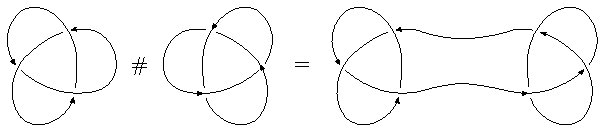
\includegraphics[scale=1.2]{figures/background/conn_sum.pdf}
  \caption{Example of the connected sum}
  \label{fig:conn-sum-example}
\end{figure}
Without orientation, it wouldn't be clear where to glue the knots back
together after cutting them. In particular: dropping the orientation
for now, we can see that we formed \cref{fig:conn-sum-example} by
attaching $u_0$ to $v_0$ in the diagram below.
\begin{figure}[H]
  \centering
  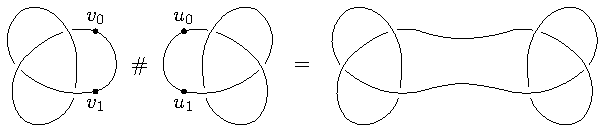
\includegraphics[scale=1.2]{figures/fundamentals/conn-sum-uo.pdf}
\end{figure}
However, without orientation to keep us in check, we could just as
well have connected $(v_0, u_1)$ and $(u_0, v_1)$. This yields two
different knots --- the former, a square knot, and the latter, a
granny knot. Hence, orientation is important!

This about wraps it up for the background. We close with some remarks
about the connected sum and how it ties in with our desire to find
more algebraic descriptions of knot structure.

\begin{proposition}
  The connected sum is commutative and well-defined for tame knots.
\end{proposition}
We'll give a sketch. If being fully rigorous, a lot of the details
here can be a pain to write out explicitly, but conceptually they are
fairly straightforward.
\begin{sproof}[Sketch]
  Given $K_0$, $K_1$, we'll show $K_0 \csum K_1$ can be ambient
  isotopied to $K_1 \csum K_0$, with arbitrary choice of cut points.

  Use ambient isotopy to turn $K_0 \csum K_1$ into a polygonal knot.
  Because it has finitely-many strands, the it doesn't get infinitely
  bunched up at any point. This intuition translates to the existence
  of a $\varepsilon > 0$ such that for any point $\msf x_0$ on $\msf
  K_0 \csum \msf K_1$, $\ol{B_{\varepsilon}(\msf x_0)}$ intersects
  $\msf K_0 \csum \msf K_1$ at exactly two points.

  Use ambient isotopy to shrink the $\msf K_1$ portion down until it's
  bounded in $B_\varepsilon(\msf x_1)$ for some $\msf x_1$ on the
  $\msf K_1$ portion of $\msf K_0 \csum \msf K_1$.\footnote{Note that
    this must be done so that the $\msf K_0$ portion remains
    unmodified.} This allows us to move the $\msf K_1$ around
  arbitrarily inside of $\msf K_0 \csum \msf K_1$. Position $\msf K_1$
  so that it is on the desired strand of $\msf K_0$ for the connected
  sum $\msf K_1 \csum K_0$. Unshrink $\msf K_1$, and then shrink $\msf
  K_0$ and apply the same process to it.
\end{sproof}
The connected sum enjoys the following properties that we will not
prove here.
\begin{proposition}~
  \begin{enumerate}
    \item $\csum$ defines a \emph{monoid} on tame knots, with the
      unknot being the identity element.
    \item Every tame knot has a unique prime factorization under
      $\csum$.
    \item The unknot cannot be written as the connected sum of two
      non-trivial knots.
  \end{enumerate}
\end{proposition}
The unique prime factorization part is particularly interesting, since
it's reminiscent of multiplication in $\ZZ$. We'd be curious to see
whether the permutation representations we introduce in the next
chapter can be used to generate an operation analogous to addition in
$\ZZ$, as this would create ring structure on tame knots.



% For the remainder of the document, we'll generally assume our knots
% are oriented.

% an operation called the
% \emph{connected sum} well-defined.
% We were unable to find a proof that went into the level of detail we
% were hoping for. We ended up proving


% We have yet to see a \emph{fully} rigorous anywhere yet
% \begin{sproof}[Sketch]

% \end{sproof}

% \begin{proof}
%   \begin{iffproof}
%     \item Each of the Reidemeister moves can be realized by elementary
%       moves. {\color{red}\huge come back and show stuff}
%     \item
%   \end{iffproof}
% \end{proof}
% {\color{red}\Huge Talk about polygonal knots}


% \noindent The proof is complicated so we won't worry about it for now.
% The point is that we now have a sense in which we can losslessly
% understand a class of \emph{knots} using a class of \emph{diagrams},
% which is big deal!

% \begin{itemize}
%   \item Discuss Haken's algorithm
%   \item Discuss other things
% \end{itemize}


%%% Local Variables:
%%% TeX-master: "../../kobayashi-thesis"
%%% End:
